\chapter{Симуляции микроскопической Kondo-ванны (R28)}
\label{chap:kondo}

Эта серия связывает феноменологический генератор из предыдущих глав с
микроскопической моделью диссипации. Нейросеть здесь не обучается. R28
сначала воспроизводит результаты двух работ Delgado и Fern\'andez-Rossier
--- каждой отдельно, разделы~\ref{sec:kondo_ss} и~\ref{sec:kondo_prb}, --- а
затем подставляет полученные операторы коллапса в тот же конвейер
``система -- каналы -- эволюция -- наблюдение -- цель'', что и в опытах A--E
(раздел~\ref{sec:kondo_demo}). Вопрос серии: как параметры среды меняют $T_2$
и $T_2^E$ при физически заданном канале.

Две работы проверяют разные части одной модели:
\begin{itemize}
\item \textbf{Статья I} --- F.~Delgado, C.~F.~Hirjibehedin,
  J.~Fern\'andez-Rossier, \emph{Consequences of Kondo exchange on quantum
  spins}, Surf.\ Sci.\ \textbf{630}, 337 (2014). Один спин: скорость
  релаксации (закон Корринги) и сдвиг уровней из-за обмена с электронами.
\item \textbf{Статья II} --- F.~Delgado, J.~Fern\'andez-Rossier,
  \emph{RKKY oscillations in the spin relaxation rates of atomic-scale
  nanomagnets}, Phys.\ Rev.\ B \textbf{95}, 075413 (2017). Несколько спинов:
  интерференция каналов распада через фазы $e^{i\mathbf q\cdot\mathbf r_l}$,
  димер, спиновые волны в цепочке, дефазировка изинговских цепочек.
\end{itemize}

\section{Общая модель}
Локализованные спины в точках $\mathbf r_l$ взаимодействуют с электронным
газом:
\[
 V=J_K\sum_l\mathbf S_l\cdot\mathbf s(\mathbf r_l),\qquad
 g=\rho_FJ_K.
\]
Во втором порядке по $g$ и в секулярном приближении скорость перехода
$|M\rangle\to|M'\rangle$ равна (статья II, ур.~20)
\begin{equation}
 \Gamma_{M\to M'}=\frac{\pi g^2}{4}G(E_M-E_{M'})
 \sum_{ll'a}K_d(k_F|\mathbf r_l-\mathbf r_{l'}|)
 \langle M'|S_l^a|M\rangle\langle M|S_{l'}^a|M'\rangle,
 \label{eq:kondo_rate}
\end{equation}
где
\[
 G(\Delta)=\frac{\Delta}{1-\exp(-\Delta/\kT)},\qquad G(0)=\kT,
\]
а пространственное ядро для электронного газа размерности $d$
\[
 K_1(x)=\cos^2x,\qquad K_2(x)=J_0(x)^2,\qquad
 K_3(x)=(\sin x/x)^2.
\]
Для одного спина ядро равно 1 и остаётся формула статьи~I; ядро ---
вклад статьи~II. Множитель $G(-\Delta)=e^{-\Delta/\kT}G(\Delta)$ обеспечивает
детальный баланс. Матрица ядра раскладывается на моды
$K_{ll'}=\sum_c\lambda_cu_{cl}u_{cl'}$; для каждого оператора
$A_{ca}=\sum_lu_{cl}S_l^a$ и боровской частоты $\omega$ строится
\[
 A_{ca}(\omega)=\sum_{E-E'=\omega}\Pi_{E'}A_{ca}\Pi_E,\qquad
 L_{ca\omega}=\sqrt{\pi g^2\lambda_cG(\omega)/4}\,A_{ca}(\omega).
\]
Сумма диссипаторов $\mathcal D[L_{ca\omega}]$ задаёт секулярный ГКСЛ
генератор. Лиувиллиан этих операторов в собственном базисе $H$ воспроизводит
скорости заселённостей и $1/T_2$ формулы~\eqref{eq:kondo_rate} с точностью
$\le10^{-14}$ (тест \file{test_collapse_dynamics_reproduce_rates_and_dephasing}),
поэтому проверки скоростей ниже относятся и к тому, что интегрирует
симулятор. Реализация: \file{src/physics/kondo_bath.py},
\file{src/blocks/channels.py}; скрипт \file{experiments/new/r28_kondo_reproduction.py}.

% ---------------------------------------------------------------------
\section{Статья I: один спин (Surf.\ Sci.\ 2014)}
\label{sec:kondo_ss}

\paragraph{Скорость релаксации.} Ур.~14--15 статьи: скорость одного спина
пропорциональна $G(\Delta)$. При $|\Delta|\ll\kT$ это закон Корринги,
$G=\kT(1+\Delta/2\kT+\dots)$, при $\Delta\gg\kT$ --- линейная зависимость от
$\Delta$. Функция $G$ сравнена с численной квадратурой электронного интеграла
$\int f(\epsilon)(1-f(\epsilon+\Delta))\,d\epsilon$ при
$\Delta/\kT\in[-6,12]$: максимальное расхождение $2.6\cdot10^{-13}$. Для
спина $1/2$ общий код даёт $\Gamma/(\pi g^2\kT/8)=1.005$ при $\Delta/\kT=0.01$;
0.5\% --- первый член разложения $G$.

\paragraph{Сдвиг уровней.} Ур.~21 статьи --- сдвиг энергии перехода через
сумму по промежуточным состояниям. Наш расчёт той же суммы двумя независимыми
способами совпадает с точностью $2.2\cdot10^{-16}$; ур.~22 (спин $1/2$)
воспроизводится.

\begin{figure}[htbp]\centering
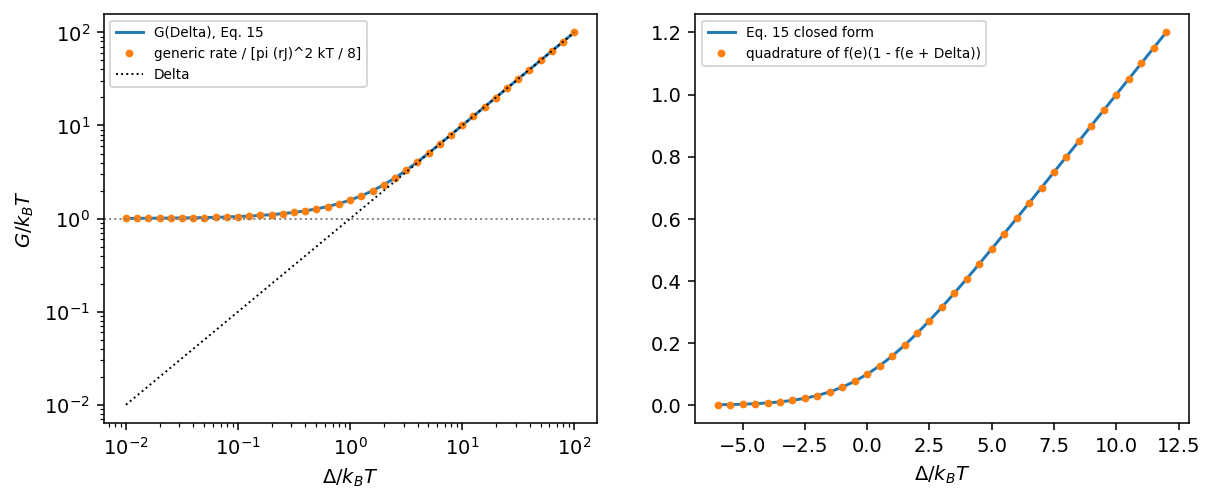
\includegraphics[width=.48\textwidth]{report_2026-11/figures/fig_surfsci_korringa.png}\hfill
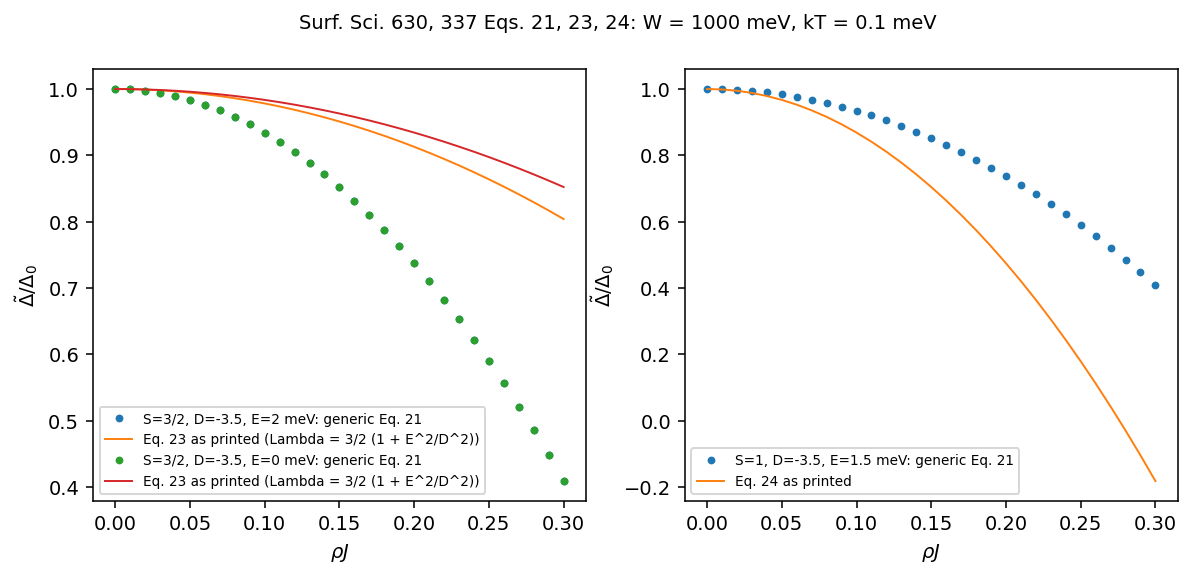
\includegraphics[width=.48\textwidth]{report_2026-11/figures/fig_surfsci_shift.png}
\caption{Статья I. Слева: $G(\Delta)$ и скорость общего кода, предел
Корринги. Справа: сдвиг энергии возбуждения по общей формуле (ур.~21)
против напечатанных частных формул (ур.~23, 24).}
\label{fig:kondo_surfsci}\end{figure}

\paragraph{Расхождения с напечатанным.} Сравнение сделано по препринт-версии
статьи; выкладки --- раздел~\ref{sec:kd}.
\begin{itemize}
\item \textbf{Ур.~23, 24.} Ур.~21 даёт
  $\tilde\Delta/\Delta=1-\tfrac34 g^2\ln(2W/\pi\kT)$ для любой квадратичной
  анизотропии и любого спина (проверено для $S=1,\tfrac32,2,\tfrac52$). Ур.~24
  печатает коэффициент $3/2$ (вдвое больше), ур.~23 --- $\Lambda/8$, то есть
  $3/16$ при $E=0$ (вчетверо меньше). Отклонение напечатанных формул от
  ур.~21 при $g\le0.3$: 0.59 (ур.~24), 0.44 и 0.40 (ур.~23, $E=0$ и 2~мэВ).
  Для $W=1$~эВ, $\kT=0.1$~мэВ уменьшение щели на 10~мэВ требует $g=0.28$ по
  общей формуле и 1.4 по ур.~23.
\item \textbf{Префактор.} Ур.~14 статьи~I содержит $\pi/2$, ур.~20
  статьи~II --- $\pi/4$; вероятно, разные соглашения для плотности
  состояний. Влияет только на абсолютный масштаб, не на отношения. Мы
  используем $\pi/4$ статьи~II: её рисунки требуют именно этой нормировки.
\end{itemize}

\begin{table}[htbp]\centering\small
\begin{tabular}{lr}
\toprule
Проверка (статья I) & max.\ откл. \\
\midrule
ур.~15: $G(\Delta)$ против квадратуры & $2.6\cdot 10^{-13}$ \\
ур.~21 против независимого расчёта той же суммы & $2.2\cdot 10^{-16}$ \\
ур.~24 с коэффициентом $3/4$ вместо напечатанного $3/2$ & $3.3\cdot 10^{-16}$ \\
\midrule
\multicolumn{2}{l}{\emph{расхождения, а не совпадения}} \\
ур.~24 как напечатано & 0.59 \\
ур.~23 как напечатано, $E=0$ и $E=2$ мэВ & 0.44 \\
\bottomrule
\end{tabular}
\caption{Статья I: максимальные отклонения
(\texttt{experiments/results/r28/deviations\_surf.csv}).}
\label{tab:kondo_ss}\end{table}

% ---------------------------------------------------------------------
\section{Статья II: несколько спинов, RKKY-осцилляции (PRB 2017)}
\label{sec:kondo_prb}

\paragraph{Димер, рис.~2 статьи.} Для двух спинов $1/2$ интерференция
каналов даёт скорость перехода триплет--синглет $\Gamma_0(1-K_d(k_Fd))$
(ур.~28, 31--32) и внутри триплета в большом поле $\Gamma_0(1+K_d(k_Fd))$
(ур.~30, 33--34). При $k_Fd=0$ первый канал подавлен (аналог
субрадиантного состояния), второй усилен вдвое. Общий код совпадает с этими
формулами на сетке из 201 точки с точностью $\le6.7\cdot10^{-16}$ при
$d=1,2,3$.

\paragraph{Спиновые волны, рис.~3.} Цепочка $S=3/2$, $D=J_H=-1$~мэВ,
трёхмерный газ, $N=4,5,6,8$. Ур.~37, $\Gamma_{SW1}(N)/\Gamma_{SW1}(1)=N$ при
$k_Fd=0$, выполнено с точностью $\le8.0\cdot10^{-15}$; вторая волна SW2 при
$k_Fd=0$ не распадается. Максимумы SW2: 1.83, 2.01, 2.23, 2.74 при
$k_Fd/\pi=0.375,\ 0.275,\ 0.25,\ 0.175$ для $N=4,5,6,8$; в статье для $N=8$
на глаз около 2.7 около 0.2.

\begin{figure}[htbp]\centering
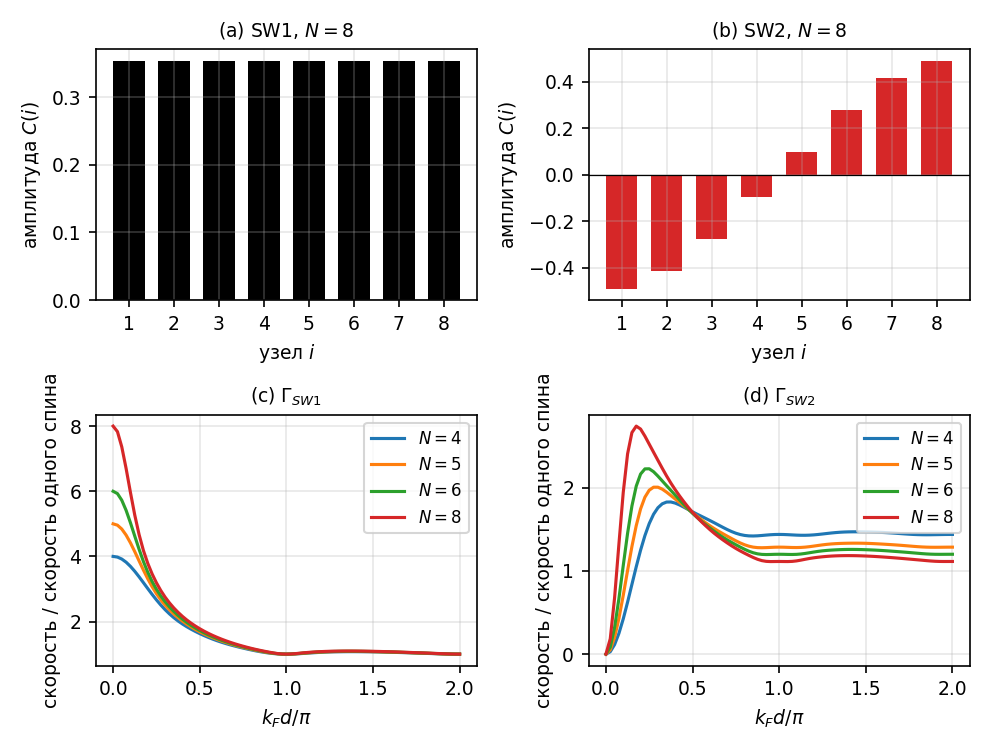
\includegraphics[width=.82\textwidth]{report_2026-11/figures/fig3_spin_waves_report.png}
\caption{Статья II, рис.~3: амплитуды и скорости распада двух нижних спиновых
волн. SW1 --- коллективное усиление однородной моды, SW2 --- подавление моды
с нулевой суммой амплитуд при $k_Fd=0$.}
\label{fig:kondo_waves}\end{figure}

\paragraph{Изинговские цепочки, рис.~4.} Дефазировка между двумя
вырожденными основными состояниями,
$\Lambda=4s^TKs$, $s_l=\pm1$. Прямой расчёт по формуле~\eqref{eq:kondo_rate}
на полном пространстве $2^N$, $N=2..8$, совпадает с суммой по ядру с
точностью $\le5.7\cdot10^{-14}$.

\paragraph{Сравнение с напечатанными рисунками.} Рисунки 2 и 4 статьи
оцифрованы из PDF (\file{paper/report_2026-11/digitize_reference.py}): кривые
выделены по цвету, вставки закрыты масками. Погрешность оцифровки видна на
кривых, которые согласуются с формулами: медиана отклонения 0.001, 95-й
процентиль $\le0.004$.

\begin{figure}[htbp]\centering
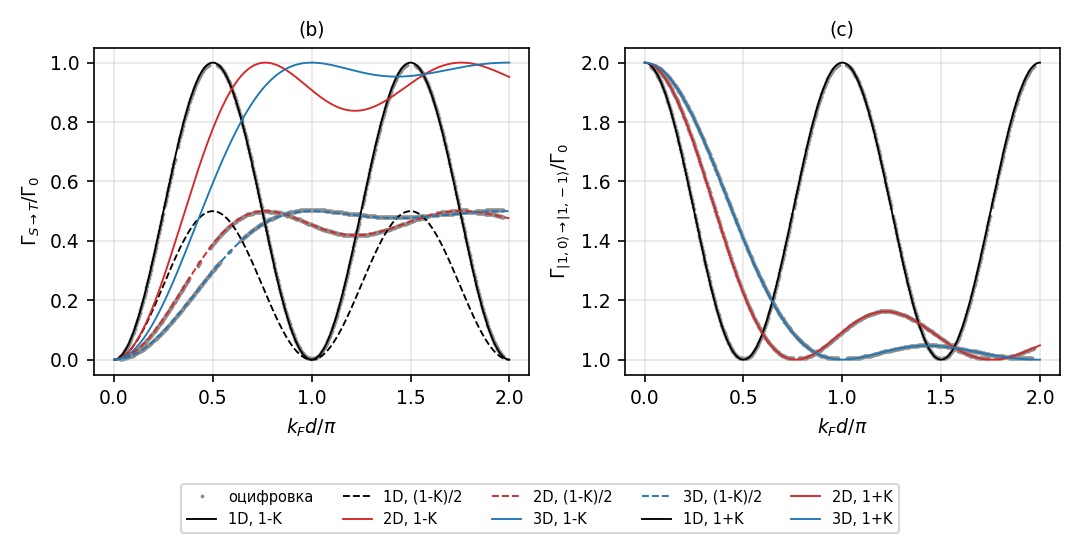
\includegraphics[width=.86\textwidth]{report_2026-11/figures/cmp_fig2.png}
\caption{Статья II, рис.~2(b, c): серые точки --- оцифровка напечатанных
кривых; линии --- наш расчёт: $1-K_d$ (сплошные), $(1-K_d)/2$ (пунктир),
$1+K_d$ (панель c).}
\label{fig:kondo_dimer}\end{figure}

\begin{figure}[htbp]\centering
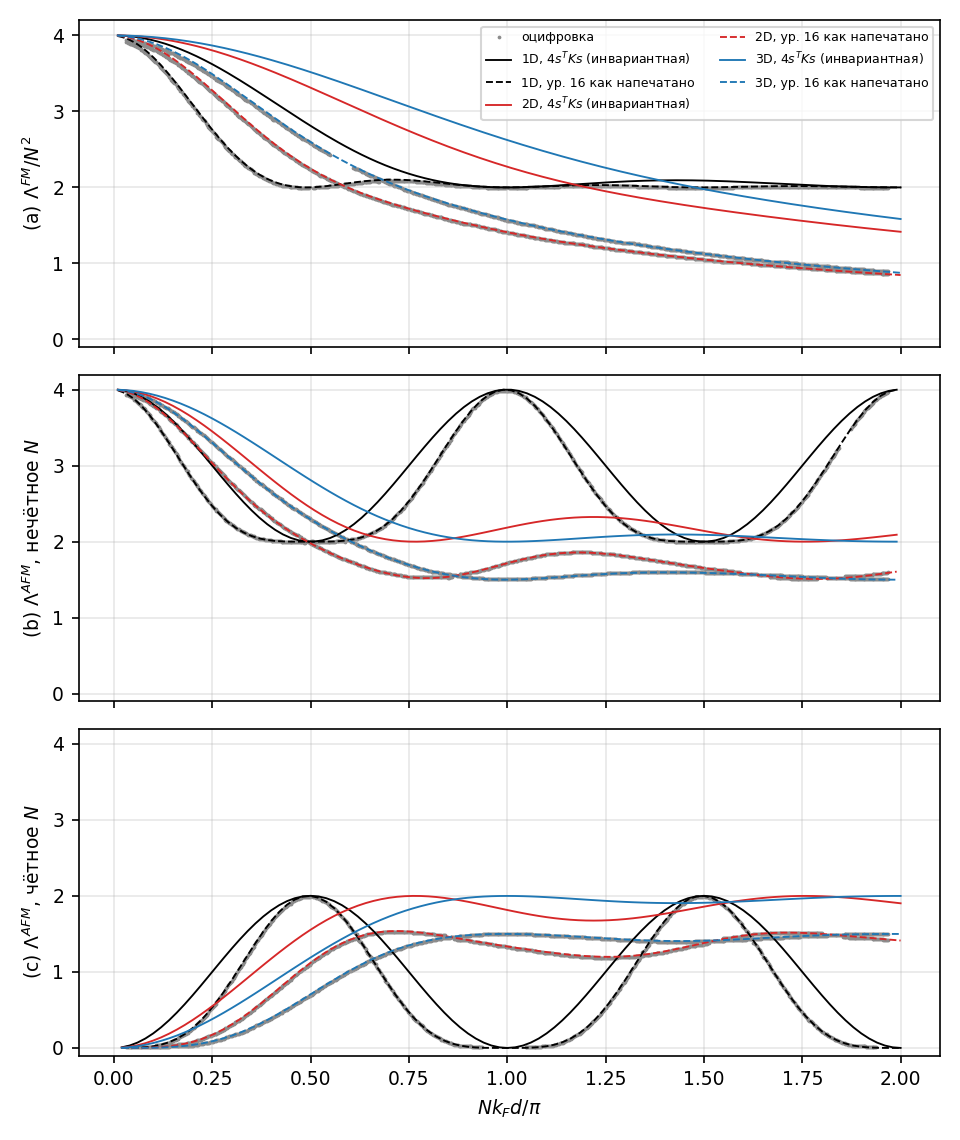
\includegraphics[width=.72\textwidth]{report_2026-11/figures/cmp_fig4.png}
\caption{Статья II, рис.~4: серые точки --- оцифровка напечатанных кривых;
сплошные --- трансляционно-инвариантная форма $4s^TKs$, пунктир --- ур.~16
статьи как напечатано (узлы $r_l=ld$). Цвета: чёрный 1D, красный 2D, синий 3D.}
\label{fig:kondo_ising}\end{figure}

\paragraph{Расхождения с напечатанным.} Выкладки --- раздел~\ref{sec:kd}.
\begin{itemize}
\item \textbf{Рис.~2(b).} Напечатанные кривые 2D и 3D равны половине
  ур.~31--32: медиана отклонения от $(1-K)/2$ 0.001 и 0.003, от самих
  уравнений 0.45 и 0.48. Кривая 1D панели (b) и все кривые панели (c)
  согласуются с уравнениями. Матричные элементы дают ур.~31--32; мы следуем им.
\item \textbf{Рис.~4.} Все девять кривых построены по ур.~16 как напечатано
  (медиана 0.005--0.018 на шкале 0--4, против 0.08--0.50 для инвариантной
  формы). Ур.~16 содержит $e^{+i\mathbf q\cdot\mathbf r}$ для одного состояния и
  $e^{-i\mathbf q\cdot\mathbf r}$ для другого и после усреднения даёт
  $2\sum s_ls_{l'}[K(k_F|r_l-r_{l'}|)+K(k_F|r_l+r_{l'}|)]$ --- результат зависит
  от начала координат. Для одного спина ур.~16 даёт $2[1+K(2k_Fr_1)]$, а
  ур.~38--39 --- 4; приложение~B (ур.~B2, B3, B6) содержит только
  $r_n-r_{n'}$. Наша форма $4s^TKs$ инвариантна. Обе совпадают при $k_Fd\to0$
  и имеют период $\pi$ в 1D; различие до 1.1 в $\Lambda^{FM}/N^2$ и 0.53 в
  $\Lambda^{AFM}$.
\item \textbf{Ур.~C4} и суммы AFM для 2D/3D как напечатано содержат
  $\xi|l-l'|$ в обоих слагаемых, то есть равны инвариантной сумме, а не
  напечатанному рисунку; по ур.~C1 второе слагаемое должно содержать
  $\xi(l+l')$, $\xi=k_Fd$.
\item \textbf{Ур.~C6} (нечётное $N$) не совпадает с суммой ур.~C1 и не
  стремится к 4 при $k_Fd\to0$. Сумма по C1:
  $\tfrac12\big[4+\big(1+\cos((2N+1)\xi)/\cos\xi\big)^2\big]$.
\end{itemize}

\begin{table}[htbp]\centering\small
\begin{tabular}{lr}
\toprule
Проверка (статья II) & max.\ откл. \\
\midrule
рис.~2(b): $1-K_d$, ур.~28, 31--32 & $5.6\cdot 10^{-16}$ \\
рис.~2(c): $1+K_d$, ур.~30, 33--34 & $6.7\cdot 10^{-16}$ \\
рис.~3: скорости SW1, SW2 против $\sum K_{ll'}C_lC_{l'}$ & $4.4\cdot 10^{-15}$ \\
ур.~37: $\Gamma_{SW1}(N)/\Gamma_{SW1}(1)=N$ & $8.0\cdot 10^{-15}$ \\
$\Lambda^{FM,AFM}$: прямой расчёт против суммы по ядру, $N=2..8$ & $5.7\cdot 10^{-14}$ \\
ур.~C3, C5, C6 (исправл.) против суммы ур.~16 & $1.5\cdot 10^{-11}$ \\
ур.~C4 как напечатано против инвариантной суммы & $2.0\cdot 10^{-11}$ \\
\midrule
\multicolumn{2}{l}{\emph{расхождения, а не совпадения}} \\
рис.~4: инвариантная форма против ур.~16, $\Lambda^{FM}/N^2$ & 1.10 \\
рис.~4: инвариантная форма против ур.~16, $\Lambda^{AFM}$ & 0.53 \\
\bottomrule
\end{tabular}
\caption{Статья II: максимальные отклонения
(\texttt{experiments/results/r28/deviations\_*.csv}).}
\label{tab:kondo_prb}\end{table}

% ---------------------------------------------------------------------
\section{Ванна Кондо в нашей задаче: два кубита}
\label{sec:kondo_demo}
Модель ванны из статей подставлена в симулятор проекта вместо
феноменологических каналов $\sigma^-$ и $\sigma^z$ со скоростью $\gamma(t)$. Системы
и цель --- те же, что в опытах A--E: два кубита XXZ и TFIM ($J=0.8$),
рассматриваемые как спины $1/2$ на расстоянии $d$; конвейер ``система --
каналы -- эволюция -- наблюдение -- цель'' не меняется, меняется только блок
каналов. Скорость затухания теперь задаётся тремя параметрами среды: $g$,
$\kT$ и $k_Fd$.

\paragraph{Постановка.} $g=0.1$, $\kT=0.2$, $t_{\max}=1200$, $\Delta t=1$;
размерность газа $d=1,2,3$; девять значений $k_Fd/\pi\in\{0,0.25,\dots,2\}$;
30 общих случайных чистых начальных состояний на точку, всего 1620 траекторий
(скрипт \file{paper/report_2026-11/kondo_demo.py}). Цели вычисляются прежними
функциями первого пересечения:
\[
 T_2=\inf\{t:C(t)\le C(0)/e\},\qquad
 T_2^E=\inf\{t:C_E(t)\le C_E(0)/e\}.
\]
Для каждой точки --- медиана по 30 траекториям и 95\%-й бутстреп-интервал
(2000 перевыборок).

\paragraph{Результаты.}
\begin{itemize}
\item \textbf{XXZ.} Медиана $T_2^E$ меняется в 4.6 раза по сетке (от 104 до
  474). В одномерном газе зависимость периодична по $k_Fd$ с периодом $\pi$
  (ядро $\cos^2k_Fd$): 474 при $k_Fd/\pi=0,1,2$ и 104 при $0.5,1.5$ --- это
  RKKY-подобные осцилляции времени декогеренции, тот же эффект интерференции,
  что в статье~II. Ширина 95\%-го интервала 6--11\% медианы, эффект
  разрешается. Цензурированных траекторий для $T_2^E$ нет.
\item \textbf{TFIM.} Изменение лишь в 1.14 раза (103--118); интервалы
  перекрываются, при 30 состояниях на точку зависимость от $k_Fd$ не
  разрешена.
\item \textbf{$T_2$ в вычислительном базисе} для XXZ определено плохо: 484
  из 810 траекторий не пересекают порог до $t_{\max}$. Причина ---
  стационарное состояние: при $\kT=0.2$ гиббсово состояние практически
  синглет (щель 3.2), его $l_1$-когерентность в вычислительном базисе равна 1,
  а порог $C(0)/e$ ниже 1 у 79\% случайных начальных состояний. Цель $T_2^E$
  этого недостатка не имеет; это ещё один довод за неё.
\end{itemize}

\begin{figure}[htbp]\centering
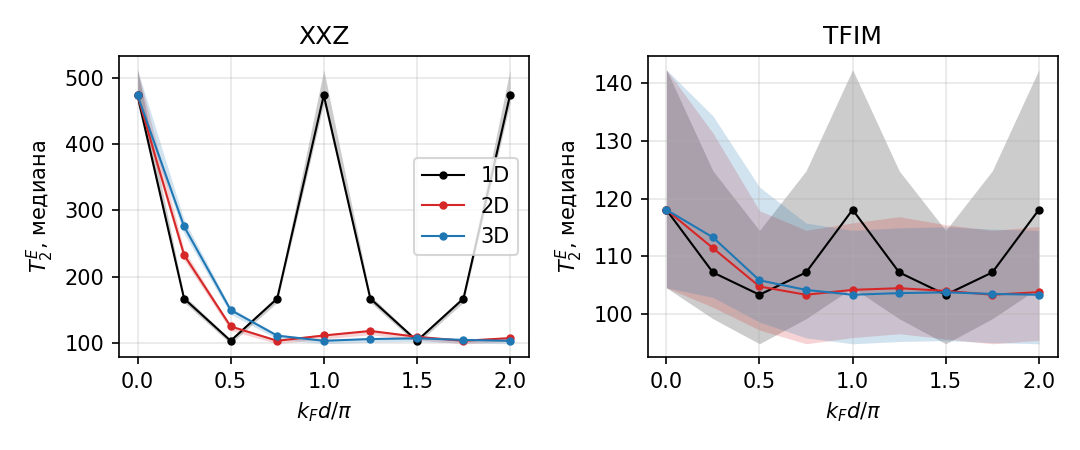
\includegraphics[width=.83\textwidth]{report_2026-11/figures/kondo_demo.png}
\caption{Ванна Кондо в задаче проекта: медиана $T_2^E$ двух кубитов и 95\%-й
бутстреп-интервал по начальным состояниям против $k_Fd/\pi$. Для XXZ
изменение расстояния разрешается, для TFIM интервал сравним со сдвигом
медианы.}
\label{fig:kondo_demo}\end{figure}

\paragraph{Зависимость от времени.} После каналов Кондо можно поставить
модификатор \texttt{bernstein\_profile} (или модуляцию OU): он умножает
скорости всех каналов на $\gamma(t)$, то есть $g^2\to g^2\gamma(t)$. Проверено
для постоянного множителя $c$: при $c=0.5$ и $c=2$ время $T_2^E$ меняется как
$1/c$ с относительной точностью $\sim10^{-4}$. Непостоянный профиль на
каналах Кондо не проверялся.

\paragraph{Что это даёт проекту.} Появляется сценарий, в котором время
декогеренции задано скрытым физическим параметром среды --- расстоянием $k_Fd$
между кубитами, --- а не произвольной кривой $\gamma(t)$. Модели прогноза на
этих данных ещё не обучались: пока получены симуляции и цель, а задача
предсказать $T_2^E$ по окну наблюдений при неизвестном $k_Fd$ --- следующий шаг.

\section{Применимость и ограничения}
При $g=0.1$ условие слабой связи выполнено; отношение максимальной скорости
затухания к минимальному ненулевому расстоянию между боровскими частотами не
превышает 0.0044 для XXZ и 0.0944 для TFIM (для TFIM запас около порядка),
так что секулярное приближение оправдано.

\paragraph{Секулярное и несекулярное уравнение.} Исключение ванны во втором
порядке по $g$ в марковском пределе даёт уравнение Блоха--Рэдфилда; в
собственном базисе $H$
\[
 \dot\rho_{ab}=-i\omega_{ab}\rho_{ab}+\sum_{cd}R_{ab,cd}\,\rho_{cd},\qquad
 \omega_{ab}=E_a-E_b .
\]
Тензор $R$ связывает все элементы $\rho$: заселённости с когерентностями и
когерентности между собой. Слагаемое $R_{ab,cd}\rho_{cd}$ с
$\omega_{cd}\ne\omega_{ab}$ осциллирует как $e^{i(\omega_{ab}-\omega_{cd})t}$ и
за время релаксации почти усредняется, если $|\omega_{ab}-\omega_{cd}|\gg\Gamma$.
Секулярное приближение отбрасывает такие слагаемые и оставляет только пары с
равными частотами. Тогда заселённости подчиняются кинетическому уравнению со
скоростями~\eqref{eq:kondo_rate}, каждая когерентность затухает со своей
скоростью $1/T_2$, а генератор имеет форму ГКСЛ, что гарантирует
положительность $\rho$; так устроены операторы $L_{ca\omega}$. Несекулярное
уравнение сохраняет полный тензор $R$: оно точнее, когда расстояния между
частотами сравнимы со скоростями, но в общем случае не имеет формы ГКСЛ и может
нарушать положительность. Отношение скорости к расстоянию между частотами,
приведённое выше, --- мера применимости секулярного приближения; для TFIM
(до 0.094) сравнение с несекулярным уравнением показало бы, насколько
приближение меняет $T_2^E$.

Чего в модели пока нет:
\begin{itemize}
\item сдвиг уровней (Lamb shift) вычисляется отдельно, но в динамику не
  включён;
\item несекулярное уравнение Блоха--Рэдфилда с секулярным ГКСЛ не сравнивалось.
\end{itemize}

% Вывод формул ванны Кондо и разбор расхождений с напечатанным.
% Подключается в отчёт (report_2026-11/report.tex) и в описание
% (kondo_simulations.tex). Требует в преамбуле \kddir и kondo_boxes.tex.

\section{Вывод формул ванны Кондо и разбор расхождений}
\label{sec:kd}

\input{\kddir kd/part1_rate.tex}
\input{\kddir kd/part2_shift.tex}
\input{\kddir kd/part3_prb.tex}
\input{\kddir kd/part4_conv.tex}


\section{Выводы}
\label{sec:kondo_conclusions}
\begin{enumerate}
\item \textbf{Модель ванны реализована и проверена.} Скорости переходов и
  дефазировки, построенные в коде, совпадают с формулами статей; динамика
  симулятора воспроизводит эти скорости с точностью $10^{-14}$.
\item \textbf{Статья I (один спин) воспроизведена.} Закон Корринги и общая
  формула сдвига уровней совпадают с нашим расчётом. Частные формулы сдвига
  (ур.~23, 24) с общей формулой той же статьи не согласуются: коэффициент
  $3/4$ против напечатанных $3/2$ и $3/16$.
\item \textbf{Статья II (несколько спинов) воспроизведена.} Формулы для
  димера, спиновых волн и изинговских цепочек совпадают с расчётом до
  машинной точности. На рис.~2(b) кривые 2D и 3D в два раза меньше формул
  статьи; рис.~4 построен по формуле, зависящей от выбора начала координат.
  Мы следуем формулам, согласованным с остальной статьёй.
\item \textbf{Модель применена к задаче проекта.} Ванна Кондо стоит в
  симуляторе вместо феноменологической $\gamma(t)$ для тех же двух кубитов
  и той же цели.
\item \textbf{Для XXZ время декогеренции зависит от расстояния между
  кубитами.} $T_2^E$ меняется в 4.6 раза и осциллирует с периодом $\pi$ по
  $k_Fd$; эффект надёжно разрешён (интервалы 6--11\%).
\item \textbf{Для TFIM зависимость слабая} (в 1.14 раза) и при 30
  начальных состояниях на точку не разрешена.
\item \textbf{Цель $T_2^E$ лучше, чем $T_2$ в вычислительном базисе:} для
  XXZ последнее плохо определено из-за почти синглетного стационарного
  состояния.
\item \textbf{Приближения выполнены:} слабая связь ($g=0.1$) и секулярное
  приближение (для TFIM с запасом около порядка).
\item \textbf{Следующий шаг:} обучить модели прогноза $T_2^E$ по окну
  наблюдений, когда параметр среды $k_Fd$ неизвестен; добавить в динамику
  сдвиг уровней и сравнить с несекулярным уравнением.
\end{enumerate}
